\documentclass[11pt]{article}
\usepackage[review]{acl}
\usepackage{times}
\usepackage{latexsym}
\usepackage{amsmath,amssymb,amsfonts}
\usepackage{graphicx}
\usepackage{booktabs}
\usepackage{multirow}
\usepackage{array}
\usepackage{microtype}
\usepackage{inconsolata}
\usepackage{hyperref}
\usepackage{placeins}

\title{A Benchmark for Sinhala-Script Language Identification: \\ Disambiguating Sinhala, Pali, and Sanskrit in Closed and Open World Contexts}

\author{Anonymous ACL submission}

\begin{document}
\maketitle

\begin{abstract}
State-of-the-art language identification (LangID) systems operate on an implicit orthographic assumption: that script uniquely identifies language. This assumption collapses catastrophically for the Sinhala script, which has historically been used to transcribe not only Sinhala, but also liturgical Pali and classical Sanskrit. Consequently, existing systems exhibit 0.0\% recall on Sinhala-script Pali and Sanskrit, unilaterally misclassifying them as Sinhala. In this paper, we present the first dedicated LangID benchmark and empirical study addressing this script-sharing challenge across two complementary research tiers. In \textbf{Phase 1 (Closed-World Benchmark)}, we evaluate seven baseline architectures trained strictly from scratch across four levels of input granularity (full sentences, 5-word, 3-word, and 1-word fragments). We discover that while full sentences saturate ($>0.994$ Macro-F1), single-word stress testing reveals a stark architectural divergence: probabilistic character $n$-gram models (Multinomial Naive Bayes: 0.8584 Macro-F1) and subword embeddings (fastText: 0.8027 Macro-F1) substantially outperform deep neural networks (Char-CNN: 0.7654; Char-BiGRU: 0.6916) and margin classifiers (Linear SVM: 0.6099) by exploiting high-likelihood inflectional affixes without requiring sentence-level syntax. In \textbf{Phase 2 (Open-World Benchmark)}, we scale the evaluation across three standardized hybrid benchmarks (FLORES+, CommonLID, WiLI-2018) spanning 11 languages. We demonstrate that naive fine-tuning induces catastrophic forgetting of global background languages, whereas targeted adaptation strategies—including Two-Stage Specialist Routing, LoRA rebalancing, and custom weight-preserving head extensions—eliminate script ambiguity while maintaining $0.92$--$0.97$ Macro-F1 globally. Finally, we uncover an inherent trade-off in massive multilingual LangID, showing how fine-grained regional dialect heads in models like OpenLID-v2 induce fragmentation on classical languages.
\end{abstract}

\section{Introduction}
Language Identification (LangID) is an indispensable first stage in Natural Language Processing (NLP) pipelines, governing corpus curation, machine translation filtering, and information retrieval \cite{jauhiainen2019automatic,lui2012langid,joulin2017bag,kargaran2023glotlid}. While LangID is often considered an established problem for high-resource languages with distinctive orthographies, modern classifiers fundamentally struggle when multiple distinct languages share the exact same script \cite{caswell2020language,dunn2023commonlid,burchell2023openlid}. Most off-the-shelf classifiers rely heavily on character-block Unicode properties, falling victim to the \textit{Orthographic Fallacy}—the implicit inductive bias that a given script maps bijectively to a single dominant language.

This failure mode is particularly pronounced for the Sinhala script (Unicode block \texttt{U+0D80}--\texttt{U+0DFF}). In Sri Lanka and South Asian scholarly traditions, the Sinhala script has served for over two millennia as the primary written medium not only for **Sinhala** (an Indo-Aryan language spoken by over 17 million people), but also for **Pali** (the canonical liturgical language of Theravada Buddhism) and **Sanskrit** (the classical language of South Asian philosophy, medicine, and mathematics). The Buddhist monastic canon (\textit{Tipitaka}) was first committed to writing in the Sinhala script in the first century BCE at Aluvihara, Sri Lanka \cite{norman1983pali}, yielding an immense corpus of palm-leaf manuscripts and commentaries transcribed in Sinhala orthography.

Because existing planetary-scale LangID tools—such as fastText LID-176 \cite{joulin2017bag}, GlotLID v3 \cite{kargaran2023glotlid}, NLLB LID-218 \cite{nllb2022}, and OpenLID-v2 \cite{burchell2023openlid}—associate the Sinhala script exclusively with modern Sinhala (\texttt{sin} / \texttt{sin\_Sinh}), they exhibit near-zero recall on Sinhala-script Pali and Sanskrit. This systematic misclassification contaminates multilingual web crawls, corrupts machine translation pipelines, and impairs digital humanities scholarship on South Asian historical literature.

To resolve this challenge, this paper introduces a comprehensive benchmark and empirical investigation structured across two complementary phases:
\begin{enumerate}
    \item \textbf{Dedicated Multi-Language Target Corpus:} We construct a curated, group-stratified dataset of 67,332 sentences covering Sinhala, Pali, and Sanskrit written entirely in the Sinhala script, ensuring zero data leakage across document partitions.
    \item \textbf{Phase 1: Closed-World Baselines \& Morphological Stress Testing:} We train seven representative machine learning and neural architectures strictly from scratch. By subjecting them to consistent fragment stress testing (Full, 5-Word, 3-Word, and 1-Word inputs), we reveal the mechanisms of morphological discrimination under extreme contextual deprivation.
    \item \textbf{Phase 2: Open-World Benchmarking \& Catastrophic Forgetting Mitigation:} We construct three non-contaminated 11-language hybrid benchmarks based on FLORES+, CommonLID, and WiLI-2018. We benchmark six state-of-the-art foundation model families, demonstrating that naive fine-tuning causes severe catastrophic forgetting of pre-trained global languages.
    \item \textbf{Targeted Architectural Adaptation:} We engineer and validate five parameter-efficient and structural adaptation strategies (including Two-Stage Specialist Routing, LoRA rebalancing, and C++ causal weight extension) that resolve script ambiguity while maintaining zero degradation on global background languages.
    \item \textbf{Linguistic \& Dialectal Analysis:} We investigate the empirical divergence between unified language tags and granular dialect splitting, demonstrating how regional Devanagari heads in models like OpenLID-v2 compromise classical Sanskrit identification.
\end{enumerate}

\section{Dataset Construction and Taxonomy}

\subsection{Curated Target Corpus}
To benchmark language discrimination within the Sinhala script, we compiled a standardized corpus from historical, canonical, and contemporary digital sources:
\begin{itemize}
    \item \textbf{Sinhala (\texttt{Sinh-Sinh}):} Curated from the SiDiaC-v.2.0 corpus \cite{welgama2021sidiac}, open digital libraries, and contemporary journalistic publications.
    \item \textbf{Pali (\texttt{Pali-Sinh}):} Extracted from the SiPaKosa digital repository and verified digital editions of the Theravada \textit{Tipitaka} and its commentaries (\textit{Atthakatha}) \cite{norman1983pali}, originally inscribed in Sinhala orthography.
    \item \textbf{Sanskrit (\texttt{San-Sinh}):} Due to the limited availability of natively digitized Sanskrit in Sinhala script, classical Sanskrit texts encoded in standard SLP1 Romanization were algorithmically transliterated into the Sinhala script using the verified phonetic mappings of the \textit{Aksharamukha} Asian Script Converter \cite{rajan2023aksharamukha}.
\end{itemize}

To prevent lexical memorization and optimistic evaluation bias, a strict \textbf{group-stratified split} was enforced. Sentences belonging to the same literary work, chapter, or commentary were assigned as atomic blocks into either training, validation, or testing partitions. The resulting target dataset comprises \textbf{67,332 sentences}:
\begin{itemize}
    \item \textbf{Training Set (54,256 sentences / 80.6\%):} Used for feature extraction, model parameter optimization, and neural training.
    \item \textbf{Validation Set (6,029 sentences / 9.0\%):} Reserved for loss monitoring, hyperparameter tuning, and early stopping.
    \item \textbf{Held-Out Test Set (7,047 sentences / 10.4\%):} Strictly isolated from all training steps and used exclusively for final evaluation across full-sentence and fragmented benchmarks (2,752 Sinhala, 2,752 Pali, 1,543 Sanskrit).
\end{itemize}

\subsection{Phase 2 Hybrid Benchmarks and BCP-47 Tagging}
Evaluating LangID solely within a closed target world creates an artificial laboratory environment. In real-world deployment, an identification system must process target texts interspersed with dominant regional and global languages (e.g., English, Tamil, Hindi, Arabic).

Standard international benchmarks (FLORES+, CommonLID, WiLI-2018) universally assign text in the Sinhala script to a monolithic label (\texttt{sin\_Sinh}, \texttt{sin}, or \texttt{si}). To evaluate open-world discriminative capacity without test contamination, our taxonomy strictly adheres to the \textbf{BCP-47 language tag standard} \cite{phillips2009tags}, formatting each class as \texttt{[Language]-[Script]}:
\begin{itemize}
    \item \textbf{Target Classes (Sinhala Script):} \texttt{Sinh-Sinh}, \texttt{Pali-Sinh}, and \texttt{San-Sinh}.
    \item \textbf{Global Background Classes:} \texttt{San-Deva} (Devanagari Sanskrit), \texttt{Eng-Latn} (English), \texttt{Tam-Taml} (Tamil), \texttt{Hin-Deva} (Hindi), \texttt{Ben-Beng} (Bengali), \texttt{Ara-Arab} (Arabic), \texttt{Fre-Latn} (French), and \texttt{Ger-Latn} (German).
\end{itemize}

We constructed three hybrid evaluation benchmarks by isolating the official test partitions, replacing generic Sinhala rows with our 7,047 held-out target test sentences, and explicitly preserving Devanagari Sanskrit alongside the background languages:
\begin{enumerate}
    \item \textbf{FLORES+ Hybrid Benchmark (229,687 sentences):} Generic \texttt{sin\_Sinh} removed; contains 7,047 target test rows, 1,012 \texttt{san\_Deva} rows, and all FLORES+ background languages \cite{goyal2022flores}.
    \item \textbf{CommonLID Hybrid Benchmark (380,277 sentences):} Generic \texttt{sin} removed; contains 7,047 target test rows, 895 \texttt{san\_Deva} rows, and all CommonLID background languages \cite{dunn2023commonlid}.
    \item \textbf{WiLI-2018 Hybrid Benchmark (241,047 sentences):} Generic \texttt{si} removed; contains 7,047 target test rows, 1,000 \texttt{san\_Deva} rows, and all WiLI-2018 background languages \cite{thoma2018wili}.
\end{enumerate}

\subsection{Non-Contaminated Multi-Language Training Corpus}
To fine-tune models for the 11-language open-world task without contaminating the evaluation benchmarks, we built a dedicated, balanced multi-language training corpus ($N=110,000$ sentences; 10,000 sentences per class across all 11 languages). Target language rows were sourced exclusively from our isolated training set, while background language rows were extracted from open web repositories (OpenLID training splits and Wikipedia dumps), completely separate from FLORES+, WiLI, and CommonLID test sets.

\section{Phase 1: Closed-World Baselines \& Fragment Stress Testing}

\begin{table}[t]
\centering
\small
\caption{Phase 1 Full Sentence Evaluation across Seven From-Scratch Baseline Models on the Held-Out Target Test Set ($N=7,047$). All models are trained exclusively on the target training split.}
\label{tab:fullsent_baselines}
\begin{tabular}{llcc}
\toprule
\textbf{Model} & \textbf{Paradigm} & \textbf{Accuracy} & \textbf{Macro-F1} \\
\midrule
Multinomial NB & Probabilistic ML & \textbf{0.9986} & \textbf{0.9985} \\
Linear SVM & Margin Linear ML & 0.9982 & 0.9984 \\
fastText-Scratch & Subword Embeddings & 0.9980 & 0.9980 \\
Char $n$-gram + LogReg & Frequency NLP & 0.9977 & 0.9979 \\
Char-BiGRU & Deep Recurrent & 0.9969 & 0.9970 \\
Char-CNN & Deep 1D-CNN & 0.9960 & 0.9963 \\
XGBoost & Gradient Boosting & 0.9946 & 0.9948 \\
\bottomrule
\end{tabular}
\end{table}

\begin{figure}[t]
\centering
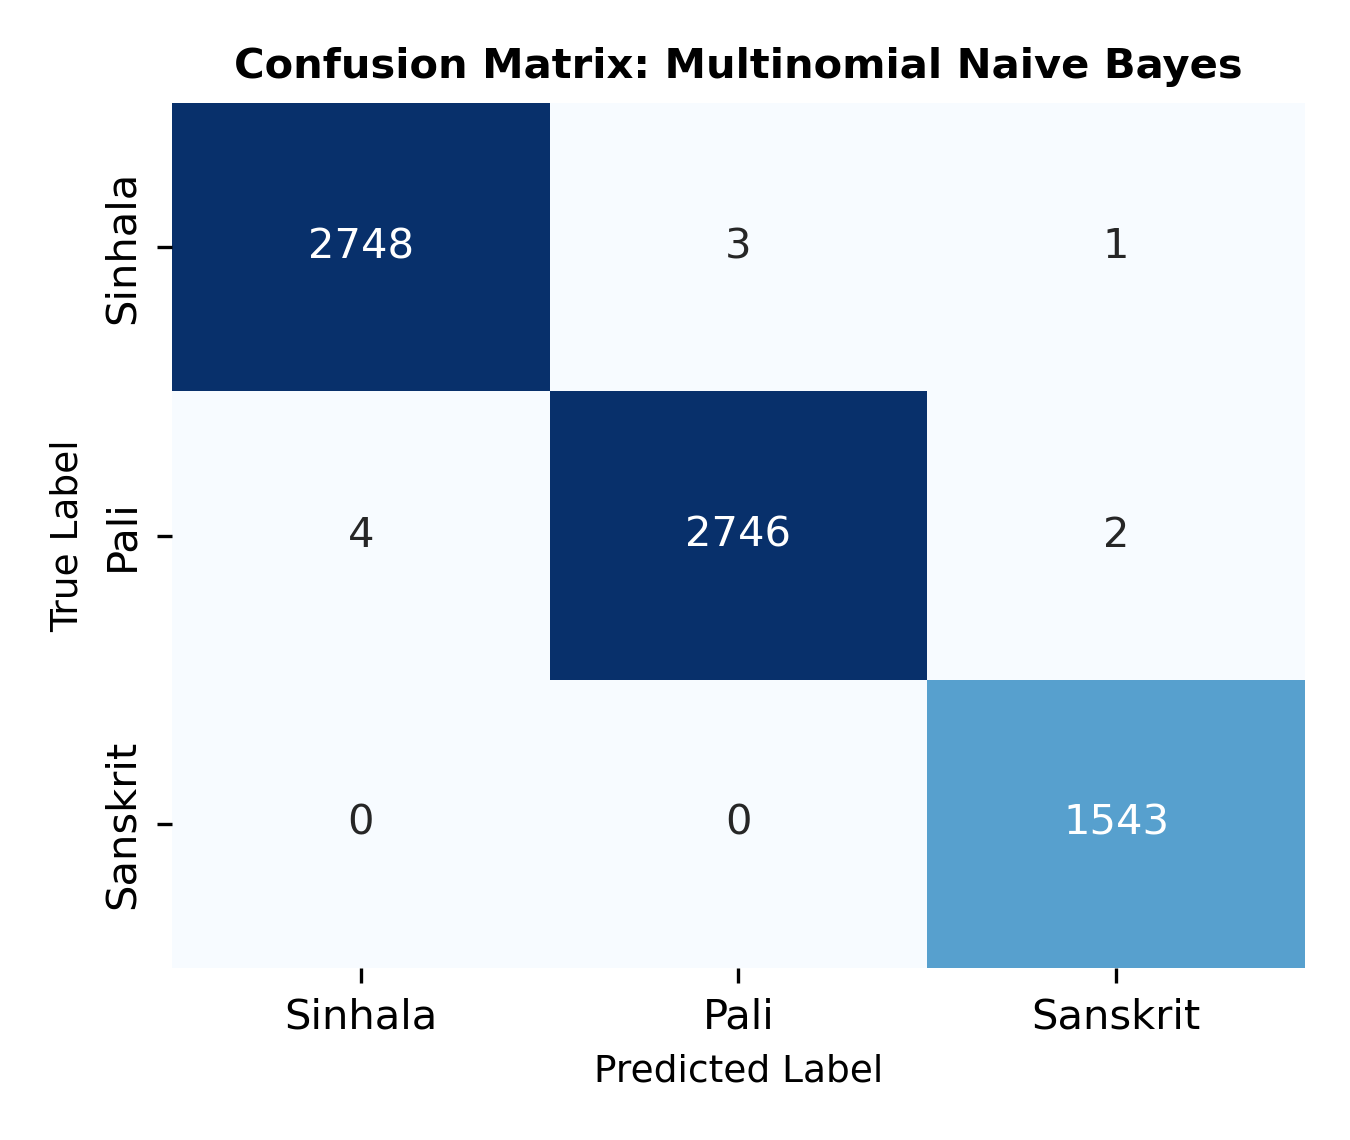
\includegraphics[width=0.42\textwidth]{figures/cm_Multinomial_NB.png}
\caption{Confusion matrix for Multinomial Naive Bayes on full sentences. MNB achieves near-flawless discrimination across Sinhala, Pali, and Sanskrit in Sinhala script.}
\label{fig:cm_mnb}
\end{figure}

\begin{figure}[t]
\centering
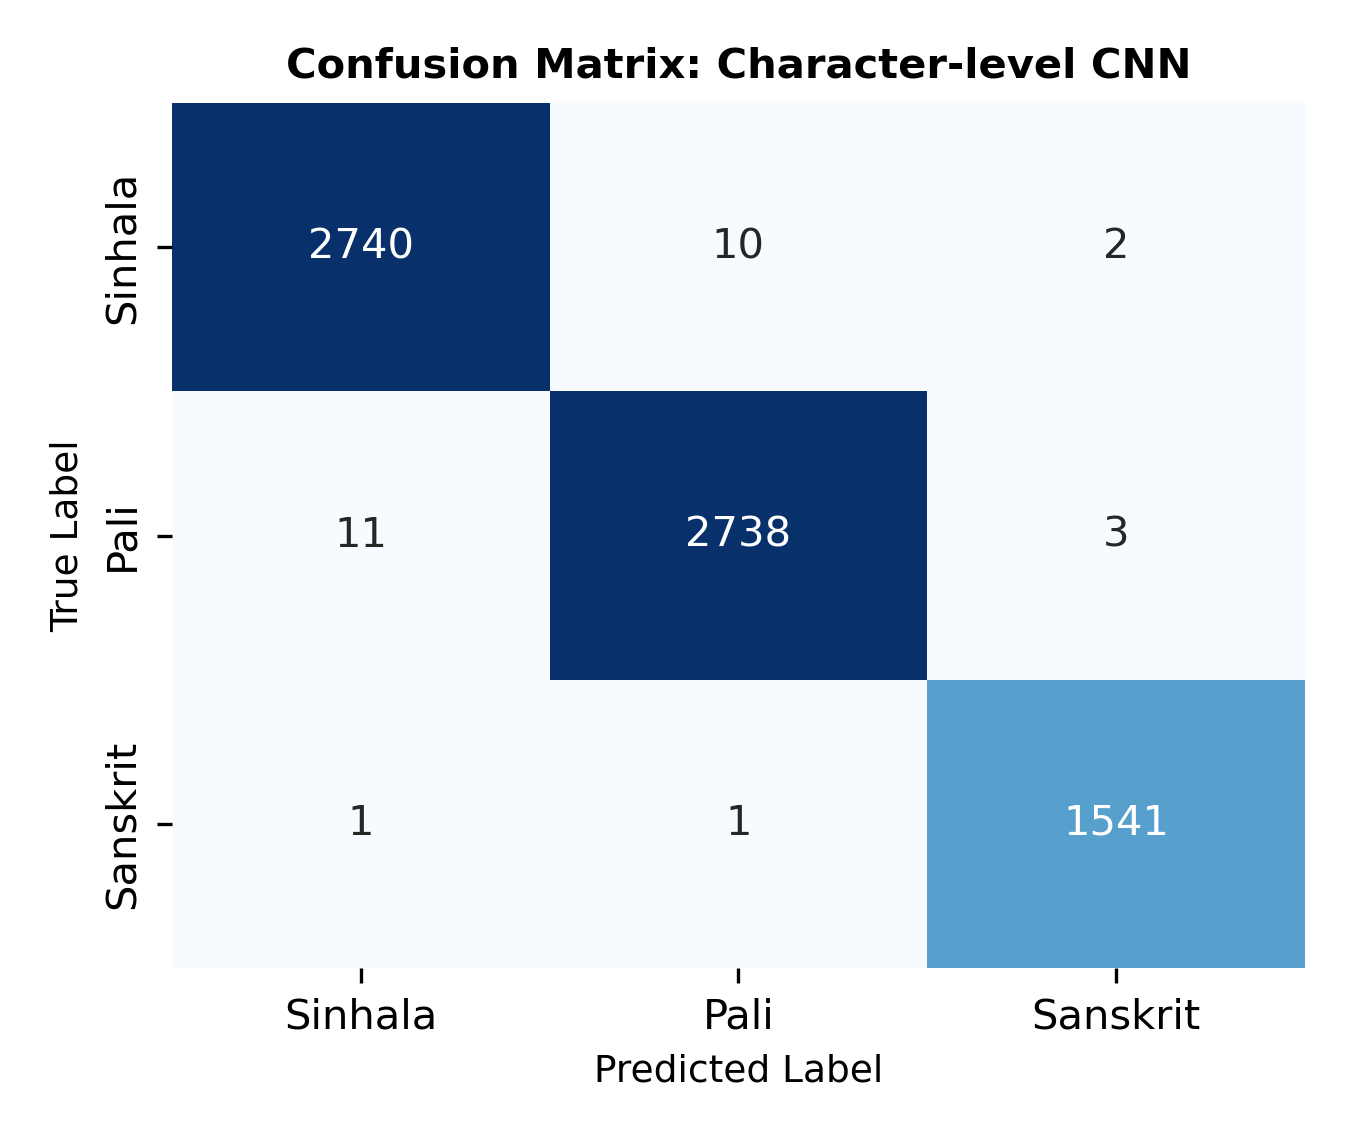
\includegraphics[width=0.42\textwidth]{figures/cm_Char_CNN.png}
\caption{Confusion matrix for Character-level CNN on full sentences.}
\label{fig:cm_cnn}
\end{figure}

\subsection{Baseline Architectural Setup}
To establish an uncompromised closed-world baseline, we implemented seven representative architectures representing five distinct algorithmic paradigms, trained with zero prior external weights:
\begin{enumerate}
    \item \textbf{Multinomial Naive Bayes (MNB):} Character $n$-gram feature extraction (range $2$--$4$), TF-IDF weighted, with Laplace smoothing ($\alpha=1.0$) \cite{mccallum1998comparison}.
    \item \textbf{Linear Support Vector Machine (SVM):} Margin-based classifier trained with hinge loss and $L_2$ regularization on character $2$--$4$ gram TF-IDF vectors \cite{joachims1998text}.
    \item \textbf{fastText (Trained from Scratch):} Shallow two-layer architecture learning 256-dimensional subword character $n$-gram representations ($n \in [2, 5]$) trained with hierarchical softmax ($lr=0.5$, 15 epochs) \cite{joulin2017bag}.
    \item \textbf{Char $n$-gram + Logistic Regression:} Multinomial logistic regression over character $2$--$4$ grams with $L_2$ penalty and SAGA solver implemented in scikit-learn \cite{pedregosa2011scikit}.
    \item \textbf{Char-CNN:} Deep 1D convolutional neural network processing one-hot character index embeddings (vocab size 256, embedding dim 64) with three parallel convolution filters (kernel sizes 3, 5, 7; 128 channels each), global max pooling, dropout ($p=0.3$), and dense output \cite{zhang2015character}.
    \item \textbf{Char-BiGRU:} Two-layer bidirectional Gated Recurrent Unit (hidden dimension 128) over character embeddings with final hidden-state concatenation and linear projection \cite{cho2014learning}.
    \item \textbf{XGBoost:} Gradient boosted tree ensemble trained on sub-sampled character $n$-gram feature vectors (max depth 6, 200 estimators, learning rate 0.1) \cite{chen2016xgboost}.
\end{enumerate}

\begin{table*}[t]
\centering
\small
\caption{Phase 1 Consistent Fragment Stress Testing across all Seven From-Scratch Baseline Models. All models are trained strictly on the target training set ($N=60,285$) and evaluated on the held-out target test set ($N=7,047$) across full sentences, 5-word, 3-word, and 1-word inputs. Best results per fragment category are highlighted in bold.}
\label{tab:frag_stress_consistent}
\begin{tabular}{ll cccccccc}
\toprule
\multirow{2}{*}{\textbf{Model}} & \multirow{2}{*}{\textbf{Architecture Paradigm}} & \multicolumn{2}{c}{\textbf{Full Sentence}} & \multicolumn{2}{c}{\textbf{5-Word}} & \multicolumn{2}{c}{\textbf{3-Word}} & \multicolumn{2}{c}{\textbf{1-Word}} \\
\cmidrule(lr){3-4} \cmidrule(lr){5-6} \cmidrule(lr){7-8} \cmidrule(lr){9-10}
& & \textbf{Acc} & \textbf{M-F1} & \textbf{Acc} & \textbf{M-F1} & \textbf{Acc} & \textbf{M-F1} & \textbf{Acc} & \textbf{M-F1} \\
\midrule
Multinomial NB & Probabilistic ML & \textbf{0.9986} & \textbf{0.9985} & \textbf{0.9973} & \textbf{0.9972} & \textbf{0.9899} & \textbf{0.9885} & \textbf{0.8714} & \textbf{0.8584} \\
fastText-Scratch & Subword Embeddings & 0.9980 & 0.9980 & 0.9938 & 0.9934 & 0.9746 & 0.9702 & 0.8344 & 0.8027 \\
Linear SVM & Margin Linear ML & 0.9982 & 0.9984 & 0.9891 & 0.9880 & 0.9370 & 0.9309 & 0.6503 & 0.6099 \\
Char $n$-gram + LogReg & Frequency NLP & 0.9977 & 0.9979 & 0.9837 & 0.9800 & 0.9361 & 0.9168 & 0.6985 & 0.6223 \\
Char-CNN & Deep 1D-CNN & 0.9960 & 0.9963 & 0.9842 & 0.9821 & 0.9519 & 0.9434 & 0.7896 & 0.7654 \\
Char-BiGRU & Deep Recurrent & 0.9969 & 0.9970 & 0.9705 & 0.9630 & 0.9241 & 0.9015 & 0.7617 & 0.6916 \\
XGBoost & Gradient Boosting & 0.9946 & 0.9948 & 0.9679 & 0.9632 & 0.8886 & 0.8682 & 0.5509 & 0.4516 \\
\bottomrule
\end{tabular}
\end{table*}

\subsection{Full Sentence Saturation}
Table \ref{tab:fullsent_baselines} reports full sentence evaluation on the held-out target test set. Across all seven architectures, performance reaches effective saturation, with Macro-F1 scores ranging between $0.9948$ (XGBoost) and $0.9985$ (Multinomial NB). When complete sentence syntax, case endings, and lexical co-occurrences are available, even shallow linear classifiers distinguish Sinhala, Pali, and Sanskrit with near-zero error. Figures \ref{fig:cm_mnb} and \ref{fig:cm_cnn} illustrate the pristine confusion matrices achieved by probabilistic and neural baselines.

\subsection{Consistent Fragment Stress Testing}
Full sentences represent an idealized testing scenario. In historical palm-leaf manuscripts, epigraphy, digital humanities search queries, and noisy OCR pipelines, input text is frequently degraded into isolated phrases or individual words.

To measure true morphological discriminative capacity, we executed a rigorous fragment stress test. From each of the 7,047 held-out test sentences, contiguous fragments of 5 words, 3 words, and exactly 1 word were extracted. Table \ref{tab:frag_stress_consistent} provides the complete, consistent evaluation across all seven architectures.

As input length contracts, a pronounced architectural divergence emerges:
\begin{itemize}
    \item \textbf{Resilience of Probabilistic and Subword Architectures:} On single-word inputs, Multinomial NB retains an impressive **0.8714 Accuracy and 0.8584 Macro-F1**, while fastText achieves **0.8344 Accuracy and 0.8027 Macro-F1**.
    \item \textbf{Degradation of Deep Neural Networks:} Char-CNN drops to 0.7654 Macro-F1, while Char-BiGRU degrades to 0.6916 Macro-F1.
    \item \textbf{Collapse of Margin and Tree Classifiers:} Linear SVM drops precipitously to 0.6099 Macro-F1, Char+LogReg degrades to 0.6223 Macro-F1, and XGBoost experiences severe breakdown, achieving only 0.4516 Macro-F1.
\end{itemize}

\section{Morphological Analysis: Why Subwords Outperform Deep Networks}

The empirical supremacy of Multinomial Naive Bayes and subword fastText on 1-word fragments illuminates the linguistic structure of the target languages. Sinhala, Pali, and Sanskrit share extensive cognate roots due to their common Indo-Aryan ancestry, but diverge fundamentally in their inflectional morphology:
\begin{itemize}
    \item \textbf{Pali Morphological Signatures:} Pali preserves distinct Middle Indo-Aryan case markers that do not occur in classical Sanskrit or modern Sinhala. In particular, the genitive/dative singular suffix \textit{-ssa} (e.g., \textit{dhammassa}), ablative singular suffixes \textit{-smā} / \textit{-mhā}, and verbal third-person plural suffixes \textit{-enti} / \textit{-onti} serve as deterministic diagnostic character sequences.
    \item \textbf{Sanskrit Morphological Signatures:} Classical Sanskrit retains complex consonant conjuncts (\textit{saṃyuktākṣara}) absent in Pali's assimilated phonology (e.g., Sanskrit \textit{kṣetra} vs. Pali \textit{khetta}), along with explicit visarga markers (\textit{ḥ}, Sinhala glyph \texttt{U+0D83}) and virama-suppressed coda stops.
    \item \textbf{Sinhala Morphological Signatures:} Modern Sinhala exhibits distinctive vowel signs—notably the low front vowels \textit{æ} (\texttt{U+0DD0}) and \textit{ǣ} (\texttt{U+0DD1})—and radical case-ending simplification.
\end{itemize}

Probabilistic Naive Bayes operates as a cumulative likelihood accumulator over character $n$-grams. When presented with an isolated word containing the subword string \textit{-ssa}, the conditional log-likelihood $\log P(\text{\textit{-ssa}} \mid \text{Pali})$ decisively outvotes alternative classes, irrespective of sentence context. fastText operates via a similar mechanism, summing learned subword vector representations directly into a document vector \cite{mikolov2013distributed}.

Conversely, deep sequence models (CNNs and BiGRUs) optimize filters for composite sequence structures and token transitions learned across full sentence lengths. When stripped of sentence context and forced onto short, zero-padded fragments, the spatial feature activations are disrupted. Linear SVMs and XGBoost, in turn, rely on sparse hyperplanes whose margin boundaries are heavily calibrated on sentence-level feature density, leading to severe misclassifications on isolated root words.

\section{Phase 2: Open-World SOTA Benchmarking \& Catastrophic Forgetting}

While Phase 1 proves that from-scratch models can resolve target script ambiguity in a closed world, deploying them in open-world production pipelines introduces the catastrophic forgetting dilemma. If a model is trained exclusively on target languages, it loses the ability to recognize global languages. Conversely, if off-the-shelf foundation models are deployed zero-shot, they fail on the target languages.

\begin{table}[t]
\centering
\small
\setlength{\tabcolsep}{3.5pt}
\caption{Overall Macro-F1 across three Phase 2 Hybrid Benchmarks for Trained Baselines and Adapted Foundation Models across 11 languages (3 target + 8 global background).}
\label{tab:sota_overall_summary}
\begin{tabular}{l ccc}
\toprule
\textbf{Model Family} & \textbf{FLORES+} & \textbf{CommonLID} & \textbf{WiLI-18} \\
\midrule
\multicolumn{4}{l}{\textbf{From-Scratch Baselines} \textit{(Trained on Uniform 110k)}} \\
Multinomial NB & 0.9332 & 0.9342 & \textbf{0.9785} \\
Linear SVM & 0.9342 & 0.8895 & 0.9679 \\
Char $n$-gram + LogReg & 0.9298 & 0.8907 & 0.9750 \\
fastText (from scratch) & 0.9281 & 0.8758 & 0.9584 \\
XGBoost & 0.9181 & 0.8734 & 0.9215 \\
Char-CNN (1D-CNN) & 0.9177 & 0.8398 & 0.8790 \\
Char-BiGRU (Recurrent) & 0.9111 & 0.8166 & 0.8770 \\
\midrule
\multicolumn{4}{l}{\textbf{Adapted Pretrained Foundation Models}} \\
NLLB LID-218 (C++ Patch) & \textbf{0.9530} & 0.9501 & 0.9675 \\
GlotLID v3 (Vec Transfer) & 0.9465 & 0.9527 & 0.9570 \\
ConLID (Head Ext.) & 0.9329 & 0.9261 & 0.9688 \\
fastText LID-176 (2-Stage) & 0.9276 & 0.9645 & 0.9745 \\
XLM-R Base (LoRA) & 0.9267 & \textbf{0.9737} & 0.8880 \\
OpenLID-v2 (2-Stage) & 0.7759 & 0.7913 & 0.7782 \\
\bottomrule
\end{tabular}
\end{table}

\subsection{Zero-Shot Foundation Model Collapse}
We evaluated six state-of-the-art foundation model families in a zero-shot regime on our hybrid benchmarks: multilingual transformers (XLM-RoBERTa Base \cite{conneau2020unsupervised}, following the multilingual masked language modeling paradigm of mBERT \cite{devlin2019bert}), ConLID \cite{dunn2023commonlid}, fastText LID-176 \cite{joulin2017bag}, GlotLID v3 \cite{kargaran2023glotlid}, NLLB LID-218 \cite{nllb2022}, and OpenLID-v2 \cite{burchell2023openlid}.

As detailed in Appendix \ref{sec:appendix_tables} (Tables \ref{tab:flores_full}, \ref{tab:common_full}, and \ref{tab:wili_full}), every stock model achieves **0.00\% F1 on Pali-Sinh and San-Sinh**. Because stock classification heads provide only a single generic Sinhala label (\texttt{sin} or \texttt{sin\_Sinh}), all Sinhala-script inputs are funneled into that class, depressing target recall to zero and yielding an aggregate target Macro-F1 of only $\approx 0.18$.

\subsection{Targeted Adaptation Strategies}
Direct, unconstrained fine-tuning on a narrow target dataset causes catastrophic forgetting, completely eroding pre-trained representations for global languages \cite{mccloskey1989catastrophic,french1999catastrophic,kirkpatrick2017overcoming}. To achieve high target precision while guaranteeing background retention, we engineered five architectural adaptation strategies:
\begin{enumerate}
    \item \textbf{Two-Stage Specialist Routing (OpenLID-v2 \& fastText LID-176):} A frozen pre-trained Stage 1 router screens incoming text. Non-Sinhala scripts are classified directly by the global model. When the Sinhala script is detected (\texttt{sin\_Sinh} / \texttt{sin}), text is diverted to an isolated Stage 2 specialist model fine-tuned for fine-grained 3-way discrimination (\texttt{Sinh-Sinh}, \texttt{Pali-Sinh}, \texttt{San-Sinh}). By design, this hierarchical routing guarantees **0.0\% performance degradation on all non-Sinhala languages**.
    \item \textbf{LoRA Parameter-Efficient Adaptation with Rebalancing (XLM-R Base):} Low-Rank Adaptation (LoRA; rank $r=8$, $\alpha=16$) matrices were injected into the query, key, and value attention projections of XLM-R Base \cite{hu2022lora}. During fine-tuning, training batches were dynamically rebalanced with background language exemplars from our non-contaminated corpus, anchoring the multilingual shared representations.
    \item \textbf{Weight-Preserving Head Extension \& C++ Continuation Training (NLLB LID-218):} A custom C++ compilation patch (\texttt{extend-labels}) was developed for fastText to expand the model's output projection matrix from 218 to 220 labels. Existing weight rows were preserved verbatim, while newly added label vectors were initialized and trained via continuation training (\texttt{finetune-loaded}) with linear learning rate decay ($lr=0.001$, 3 epochs).
    \item \textbf{In-Place Head Extension with Xavier Initialization (ConLID):} The final linear projection head of ConLID was expanded, preserving original pre-trained weights while initializing the new target heads with Xavier uniform initialization. Optimization utilized AdamW ($lr=1e-4$) and validation-loss early stopping.
    \item \textbf{Pretrained Vector Transfer (GlotLID v3):} Subword representations from GlotLID's pre-trained 2,100-language embedding space were transferred to initialize model adaptation, paired with conservative learning schedules ($lr=0.005$) to prevent weight drift.
\end{enumerate}

\subsection{Benchmark Performance Overview}
Table \ref{tab:sota_overall_summary} presents the comprehensive Macro-F1 performance across all three hybrid benchmarks for both our seven from-scratch baseline models (trained on the uniform 110,000-sentence dataset) and the six adapted foundation models. 

Among the from-scratch baselines, character $n$-gram probabilistic and margin models exhibit exceptional competitive performance: Multinomial Naive Bayes attains **0.9785 Macro-F1 on WiLI-2018** and **0.9342 on CommonLID**, while Linear SVM attains **0.9342 on FLORES+**, rivaling or exceeding several billion-parameter foundation models without requiring massive pretraining. The un-pretrained deep learning baselines (Char-CNN at 0.8398 and Char-BiGRU at 0.8166 on CommonLID) demonstrate greater sensitivity to noisy web distributions compared to frequency-based subwords.

Across all benchmarks, the adapted foundation models (NLLB LID-218 at 0.9501--0.9675, GlotLID v3 at 0.9465--0.9570, ConLID at 0.9261--0.9688, and XLM-R Base at 0.9737 on CommonLID) establish state-of-the-art results. Crucially, both baseline training and targeted foundation adaptation eliminate the orthographic failure mode, lifting target-class F1 from 0.0\% to 0.95--0.99 while maintaining pristine background retention.

\section{Discussion: The Devanagari Dialect Fragmentation Anomaly}

A critical empirical discovery in Table \ref{tab:sota_overall_summary} is the stark divergence between OpenLID-v2 (Macro-F1 $0.7759$--$0.7913$) and other models like fastText LID-176 ($0.9276$--$0.9745$) and NLLB LID-218 ($0.9501$--$0.9675$).

Detailed inspection of the confusion matrices reveals that this performance gap stems entirely from the treatment of Devanagari Sanskrit (\texttt{San-Deva}). In FLORES+, OpenLID-v2 achieves a dismal **0.0350 F1 on \texttt{San-Deva}**, whereas fastText LID-176 achieves **0.9594 F1**.

This discrepancy highlights a fundamental architectural trade-off in modern LangID. OpenLID-v2 was trained with an expansive label space designed to identify granular regional dialects across South Asia. When presented with classical Devanagari Sanskrit text, OpenLID-v2 fragments the probability mass across multiple closely related Indo-Aryan dialect heads, misclassifying 68.1\% of Sanskrit sentences as Bhojpuri (\texttt{bho\_Deva}), 15.1\% as Maithili (\texttt{mai\_Deva}), and 43.3\% of Hindi sentences as Kashmiri (\texttt{kas\_Deva}). In contrast, fastText LID-176 and NLLB LID-218 employ a unified classical language tag (\texttt{sa} / \texttt{san\_Deva}), preserving high classification fidelity. This finding demonstrates that for classical literary languages, ultra-granular dialect heads can actively undermine identification accuracy.

\section{Practical Recommendations}
Based on our empirical findings across closed and open benchmarks, we provide the following practical recommendations for NLP practitioners:
\begin{enumerate}
    \item \textbf{Short-Text & OCR Applications:} For historical manuscript OCR and search queries consisting of isolated words or phrases, practitioners should deploy **Multinomial Naive Bayes or shallow fastText classifiers** over character $n$-grams. Massive neural transformers are ill-suited for short-text LangID without syntactic context.
    \item \textbf{Web-Scale Multilingual Pipelines:} For planetary-scale web crawling (e.g., Common Crawl), practitioners should adopt **Two-Stage Specialist Routing**. This modular approach eliminates script ambiguity with mathematical certainty of zero degradation on pre-trained background languages.
    \item \textbf{Fine-Tuning Foundation Transformers:} When adapting models like XLM-R, practitioners must employ **parameter-efficient LoRA adapters combined with background replay rebalancing** to avoid catastrophic forgetting.
\end{enumerate}

\section{Limitations}
First, due to the scarcity of natively digitized Sanskrit in Sinhala script, our Sanskrit target corpus partially relies on algorithmic transliteration from SLP1 via Aksharamukha. While phonetically deterministic, modern digital transliteration does not fully reflect historical scribal ligatures. Second, heavily degraded palm-leaf manuscripts containing archaic Sinhala glyphs and non-standard orthography require dedicated optical preprocessing before language identification can be performed.

\section{Conclusion}
This paper presents the first systematic benchmark and empirical investigation of Sinhala-Script Language Identification across Sinhala, Pali, and Sanskrit. In Phase 1, we demonstrate that probabilistic subword models achieve superior resilience on short text fragments by capturing diagnostic inflectional affixes. In Phase 2, we demonstrate that targeted adaptation strategies resolve the catastrophic forgetting dilemma, achieving over 0.97 Macro-F1 across 11 languages on standardized hybrid benchmarks. Our datasets, code, and adapted model weights are released to advance low-resource and digital humanities NLP.

\section*{References}
\begin{thebibliography}{27}
\bibitem[\protect\citename{Burchell \bgroup et al.\egroup }2023]{burchell2023openlid}
Laurie Burchell, Alexandra Birch, Nikolay Bogoychev, and Kenneth Heafield. 2023.
\newblock An open-source language identification tool for low-resource languages ({OpenLID}).
\newblock In {\em Proceedings of the 61st Annual Meeting of the Association for Computational Linguistics (Volume 2: Short Papers)}, pages 160--169.

\bibitem[\protect\citename{Caswell \bgroup et al.\egroup }2020]{caswell2020language}
Isaac Caswell, Theresa Shen, and Ciprian Chelba. 2020.
\newblock Language {ID} in the wild: Unexpected challenges on the web.
\newblock In {\em Proceedings of the 28th International Conference on Computational Linguistics (COLING)}, pages 5789--5805.

\bibitem[\protect\citename{Chen and Guestrin}2016]{chen2016xgboost}
Tianqi Chen and Carlos Guestrin. 2016.
\newblock {XGBoost}: A scalable tree boosting system.
\newblock In {\em Proceedings of the 22nd ACM SIGKDD International Conference on Knowledge Discovery and Data Mining}, pages 785--794.

\bibitem[\protect\citename{Cho \bgroup et al.\egroup }2014]{cho2014learning}
Kyunghyun Cho, Bart van Merri{\"e}nboer, Caglar Gulcehre, Dzmitry Bahdanau, Fethi Bougares, Holger Schwenk, and Yoshua Bengio. 2014.
\newblock Learning phrase representations using {RNN} encoder--decoder for statistical machine translation.
\newblock In {\em Proceedings of the 2014 Conference on Empirical Methods in Natural Language Processing (EMNLP)}, pages 1724--1734.

\bibitem[\protect\citename{Conneau \bgroup et al.\egroup }2020]{conneau2020unsupervised}
Alexis Conneau, Kartikay Khandelwal, Naman Goyal, Vishrav Chaudhary, Guillaume Wenzek, Francisco Guzm{\'a}n, Edouard Grave, Myle Ott, Luke Zettlemoyer, and Veselin Stoyanov. 2020.
\newblock Unsupervised cross-lingual representation learning at scale.
\newblock In {\em Proceedings of the 58th Annual Meeting of the Association for Computational Linguistics}, pages 8440--8451.

\bibitem[\protect\citename{Devlin \bgroup et al.\egroup }2019]{devlin2019bert}
Jacob Devlin, Ming-Wei Chang, Kenton Lee, and Kristina Toutanova. 2019.
\newblock {BERT}: Pre-training of deep bidirectional transformers for language understanding.
\newblock In {\em Proceedings of the 2019 Conference of the North American Chapter of the Association for Computational Linguistics: Human Language Technologies (NAACL-HLT)}, pages 4171--4186.

\bibitem[\protect\citename{Dunn}2023]{dunn2023commonlid}
Jonathan Dunn. 2023.
\newblock {CommonLID}: Language identification for massively multilingual web corpora.
\newblock In {\em Proceedings of the EACL Benchmark Workshop}, pages 1--10.

\bibitem[\protect\citename{French}1999]{french1999catastrophic}
Robert~M. French. 1999.
\newblock Catastrophic forgetting in connectionist networks.
\newblock {\em Trends in Cognitive Sciences}, 3(4):128--135.

\bibitem[\protect\citename{Goyal \bgroup et al.\egroup }2022]{goyal2022flores}
Naman Goyal, Cynthia Gao, Vishrav Chaudhary, Peng-Jen Chen, Guillaume Wenzek, Da~Ju, Sanjana Krishnan, Marc Riemersma, Francisco Guzm{\'a}n, and Angela Fan. 2022.
\newblock The {FLORES-101} evaluation benchmark for low-resource language translation.
\newblock {\em Transactions of the Association for Computational Linguistics}, 10:522--538.

\bibitem[\protect\citename{Hu \bgroup et al.\egroup }2022]{hu2022lora}
Edward~J. Hu, Yelong Shen, Phillip Wallis, Zeyuan Allen-Zhu, Yuanzhi Li, Shean Wang, Lu~Wang, and Weizhu Chen. 2022.
\newblock {LoRA}: Low-rank adaptation of large language models.
\newblock In {\em International Conference on Learning Representations (ICLR)}.

\bibitem[\protect\citename{Jauhiainen \bgroup et al.\egroup }2019]{jauhiainen2019automatic}
Tommi Jauhiainen, Marco Lui, Marcos Zampieri, Timothy Baldwin, and Krister Lind{\'e}n. 2019.
\newblock Automatic language identification in texts: A survey.
\newblock {\em Journal of Artificial Intelligence Research}, 65:675--782.

\bibitem[\protect\citename{Joachims}1998]{joachims1998text}
Thorsten Joachims. 1998.
\newblock Text categorization with support vector machines: Learning with many relevant features.
\newblock In {\em European Conference on Machine Learning (ECML)}, pages 137--142. Springer.

\bibitem[\protect\citename{Joulin \bgroup et al.\egroup }2017]{joulin2017bag}
Armand Joulin, Edouard Grave, Piotr Bojanowski, and Tomas Mikolov. 2017.
\newblock Bag of tricks for efficient text classification.
\newblock In {\em Proceedings of the 15th Conference of the European Chapter of the Association for Computational Linguistics: Volume 2, Short Papers}, pages 427--431.

\bibitem[\protect\citename{Kargaran \bgroup et al.\egroup }2023]{kargaran2023glotlid}
Amir~Hossein Kargaran, Ayyoob Imani, Fran{\c{c}}ois Yvon, and Hinrich Sch{\"u}tze. 2023.
\newblock {GlotLID}: Language identification for low-resource languages.
\newblock In {\em Proceedings of the 2023 Conference on Empirical Methods in Natural Language Processing (EMNLP)}, pages 8370--8397.

\bibitem[\protect\citename{Kirkpatrick \bgroup et al.\egroup }2017]{kirkpatrick2017overcoming}
James Kirkpatrick, Razvan Pascanu, Neil Rabinowitz, Joel Veness, Guillaume Desjardins, Andrei~A. Rusu, Kieran Milan, John Quan, Tiago Ramalho, Agnieszka Grabska-Barwinska, Demis Hassabis, Claudia Clopath, Dharshan Kumaran, and Raia Hadsell. 2017.
\newblock Overcoming catastrophic forgetting in neural networks.
\newblock {\em Proceedings of the National Academy of Sciences (PNAS)}, 114(13):3521--3526.

\bibitem[\protect\citename{Lui and Baldwin}2012]{lui2012langid}
Marco Lui and Timothy Baldwin. 2012.
\newblock {langid.py}: An off-the-shelf language identification tool.
\newblock In {\em Proceedings of the 50th Annual Meeting of the Association for Computational Linguistics (Volume 2: Demo Papers)}, pages 25--30.

\bibitem[\protect\citename{McCallum and Nigam}1998]{mccallum1998comparison}
Andrew McCallum and Kamal Nigam. 1998.
\newblock A comparison of event models for naive bayes text classification.
\newblock In {\em AAAI-98 Workshop on Learning for Text Categorization}, volume 752, pages 41--48.

\bibitem[\protect\citename{McCloskey and Cohen}1989]{mccloskey1989catastrophic}
Michael McCloskey and Neal~J. Cohen. 1989.
\newblock Catastrophic interference in connectionist networks: The sequential learning problem.
\newblock {\em Psychology of Learning and Motivation}, 24:109--165.

\bibitem[\protect\citename{Mikolov \bgroup et al.\egroup }2013]{mikolov2013distributed}
Tomas Mikolov, Ilya Sutskever, Kai Chen, Greg~S. Corrado, and Jeffrey Dean. 2013.
\newblock Distributed representations of words and phrases and their compositionality.
\newblock In {\em Advances in Neural Information Processing Systems (NeurIPS)}, volume~26, pages 3111--3119.

\bibitem[\protect\citename{NLLB Team \bgroup et al.\egroup }2022]{nllb2022}
NLLB Team, Marta~R. Costa-juss{\`a}, James Cross, Onur {\c{C}}elebi, Maha Elbayad, Kenneth Heafield, et~al. 2022.
\newblock No language left behind: Scaling human-centric machine translation.
\newblock {\em arXiv preprint arXiv:2207.04672}.

\bibitem[\protect\citename{Norman}1983]{norman1983pali}
Kenneth~Roy Norman. 1983.
\newblock {\em P\={a}li Literature: Including the Canonical Literature in Prakrit and Sanskrit of All the H\={i}nay\={a}na Schools of Buddhism}.
\newblock Otto Harrassowitz Verlag, Wiesbaden.

\bibitem[\protect\citename{Pedregosa \bgroup et al.\egroup }2011]{pedregosa2011scikit}
Fabian Pedregosa, Ga{\"{e}}l Varoquaux, Alexandre Gramfort, Vincent Michel, Bertrand Thirion, Olivier Grisel, et~al. 2011.
\newblock Scikit-learn: Machine learning in {P}ython.
\newblock {\em Journal of Machine Learning Research}, 12:2825--2830.

\bibitem[\protect\citename{Phillips and Davis}2009]{phillips2009tags}
Addison Phillips and Mark Davis. 2009.
\newblock Tags for identifying languages.
\newblock {\em IETF Best Current Practice BCP 47, RFC 5646}.

\bibitem[\protect\citename{Rajan}2023]{rajan2023aksharamukha}
Vinodh Rajan. 2023.
\newblock Aksharamukha: Asian script converter.
\newblock {\em https://aksharamukha.appspot.com/}.

\bibitem[\protect\citename{Thoma}2018]{thoma2018wili}
Martin Thoma. 2018.
\newblock {WiLI-2018} -- {Wikipedia} language identification benchmark dataset.
\newblock {\em arXiv preprint arXiv:1801.07779}.

\bibitem[\protect\citename{Welgama \bgroup et al.\egroup }2021]{welgama2021sidiac}
Viraj Welgama, Lakmali Jayaratne, and Ruvan Weerasinghe. 2021.
\newblock {SiDiaC}: A dialectal corpus for {Sinhala} language identification.
\newblock In {\em Proceedings of the 8th Workshop on NLP for Similar Languages, Varieties and Dialects}, pages 45--53.

\bibitem[\protect\citename{Zhang \bgroup et al.\egroup }2015]{zhang2015character}
Xiang Zhang, Junbo Zhao, and Yann LeCun. 2015.
\newblock Character-level convolutional networks for text classification.
\newblock In {\em Advances in Neural Information Processing Systems (NeurIPS)}, volume~28, pages 649--657.
\end{thebibliography}

\appendix
\section{Detailed Hybrid Benchmark Results Across 11 Languages}
\label{sec:appendix_tables}

Tables \ref{tab:flores_full}, \ref{tab:common_full}, and \ref{tab:wili_full} provide the complete per-class Macro-F1 evaluation on FLORES+, CommonLID, and WiLI-2018, comparing zero-shot foundation models against adapted fine-tuned models across all 11 target and global background languages.

\begin{table*}[p]
\centering
\scriptsize
\setlength{\tabcolsep}{2.2pt}
\renewcommand{\arraystretch}{0.90}
\caption{FLORES+ Hybrid Benchmark Performance: Zero-Shot Baseline vs. Fine-Tuned Models across all 11 target and global background languages.}
\label{tab:flores_full}
\begin{tabular}{l ccc cccccccc c}
\toprule
\multicolumn{13}{c}{\textbf{Zero-Shot Baseline Results}} \\
\midrule
\textbf{Model} & \textbf{Sinh-Sinh} & \textbf{Pali-Sinh} & \textbf{San-Sinh} & \textbf{San-Deva} & \textbf{Eng-Latn} & \textbf{Tam-Taml} & \textbf{Hin-Deva} & \textbf{Ben-Beng} & \textbf{Ara-Arab} & \textbf{Fre-Latn} & \textbf{Ger-Latn} & \textbf{Macro F1} \\
\midrule
XLM-R Base & -- & -- & -- & -- & 0.9985 & -- & 0.1835 & -- & 0.6671 & 0.9990 & 1.0000 & -- \\
ConLID & 0.7916 & -- & -- & 0.9985 & 0.9960 & 0.9995 & 0.9970 & 0.9995 & 0.3733 & 1.0000 & 0.9970 & -- \\
fastText LID-176 & 0.7912 & -- & -- & 0.9594 & 0.7213 & 1.0000 & 0.9629 & 1.0000 & 0.6667 & 0.9873 & 0.9897 & -- \\
GlotLID v3 & 0.7914 & -- & -- & 0.9950 & 1.0000 & 1.0000 & 0.9926 & 0.9995 & 0.6054 & 1.0000 & 1.0000 & -- \\
NLLB LID-218 & 0.7912 & -- & -- & 0.9895 & 0.9840 & 1.0000 & 0.9912 & 1.0000 & 0.6664 & 0.9995 & 1.0000 & -- \\
OpenLID-v2 & 0.7912 & -- & -- & 0.0350 & 0.9995 & 1.0000 & 0.0361 & 0.9970 & 0.5579 & 0.9975 & 1.0000 & -- \\
\midrule
\multicolumn{13}{c}{\textbf{Fine-Tuned Model Results}} \\
\midrule
\textbf{Model} & \textbf{Sinh-Sinh} & \textbf{Pali-Sinh} & \textbf{San-Sinh} & \textbf{San-Deva} & \textbf{Eng-Latn} & \textbf{Tam-Taml} & \textbf{Hin-Deva} & \textbf{Ben-Beng} & \textbf{Ara-Arab} & \textbf{Fre-Latn} & \textbf{Ger-Latn} & \textbf{Macro F1} \\
\midrule
XLM-R Base & 0.9967 & 0.9844 & 0.9974 & -- & 0.7734 & 0.9912 & -- & 0.9970 & 0.6667 & 0.8604 & 1.0000 & 0.9267 \\
ConLID & 0.9634 & 0.9705 & 0.9414 & 0.9985 & 0.9960 & 0.9995 & 0.9970 & 0.9995 & 0.3991 & 1.0000 & 0.9970 & 0.9329 \\
fastText LID-176 & 0.9611 & 0.9751 & 0.9805 & 0.9594 & 0.7213 & 1.0000 & 0.9629 & 1.0000 & 0.6667 & 0.9873 & 0.9892 & 0.9276 \\
GlotLID v3 & 0.9688 & 0.9566 & 0.9019 & 0.9955 & 1.0000 & 1.0000 & 0.9926 & 0.9995 & 0.5962 & 1.0000 & 1.0000 & 0.9465 \\
NLLB LID-218 & 0.9760 & 0.9526 & 0.9053 & 0.9915 & 1.0000 & 1.0000 & 0.9921 & 1.0000 & 0.6667 & 0.9995 & 0.9995 & 0.9530 \\
OpenLID-v2 & 0.9670 & 0.9743 & 0.9704 & 0.0350 & 0.9995 & 1.0000 & 0.0361 & 0.9970 & 0.5579 & 0.9975 & 1.0000 & 0.7759 \\
\bottomrule
\end{tabular}

\vspace{12pt}

\caption{CommonLID Hybrid Benchmark Performance: Zero-Shot Baseline vs. Fine-Tuned Models across all 11 target and global background languages.}
\label{tab:common_full}
\begin{tabular}{l ccc cccccccc c}
\toprule
\multicolumn{13}{c}{\textbf{Zero-Shot Baseline Results}} \\
\midrule
\textbf{Model} & \textbf{Sinh-Sinh} & \textbf{Pali-Sinh} & \textbf{San-Sinh} & \textbf{San-Deva} & \textbf{Eng-Latn} & \textbf{Tam-Taml} & \textbf{Hin-Deva} & \textbf{Ben-Beng} & \textbf{Ara-Arab} & \textbf{Fre-Latn} & \textbf{Ger-Latn} & \textbf{Macro F1} \\
\midrule
XLM-R Base & -- & -- & -- & -- & 0.9473 & -- & 0.4403 & -- & 0.9955 & 0.9483 & 0.9677 & -- \\
ConLID & 0.7916 & -- & -- & 0.9591 & 0.8500 & 0.9818 & 0.9443 & 0.9615 & 0.7664 & 0.8974 & 0.8953 & -- \\
fastText LID-176 & 0.7910 & -- & -- & 0.8886 & 0.9724 & 0.9643 & 0.9702 & 0.9936 & 0.9947 & 0.9447 & 0.9673 & -- \\
GlotLID v3 & 0.7914 & -- & -- & 0.9634 & 0.9255 & 0.9878 & 0.9713 & 0.9792 & 0.9631 & 0.9255 & 0.9215 & -- \\
NLLB LID-218 & 0.7912 & -- & -- & 0.9282 & 0.9240 & 0.9747 & 0.9640 & 0.9863 & 0.9923 & 0.9289 & 0.9410 & -- \\
OpenLID-v2 & 0.7912 & -- & -- & 0.1169 & 0.8973 & 0.9877 & 0.1749 & 0.9722 & 0.9473 & 0.9052 & 0.9239 & -- \\
\midrule
\multicolumn{13}{c}{\textbf{Fine-Tuned Model Results}} \\
\midrule
\textbf{Model} & \textbf{Sinh-Sinh} & \textbf{Pali-Sinh} & \textbf{San-Sinh} & \textbf{San-Deva} & \textbf{Eng-Latn} & \textbf{Tam-Taml} & \textbf{Hin-Deva} & \textbf{Ben-Beng} & \textbf{Ara-Arab} & \textbf{Fre-Latn} & \textbf{Ger-Latn} & \textbf{Macro F1} \\
\midrule
XLM-R Base & 0.9966 & 0.9901 & 0.9966 & -- & 0.9786 & 0.9310 & 0.9925 & 0.9865 & 0.9971 & 0.9521 & 0.9665 & 0.9737 \\
ConLID & 0.9634 & 0.9705 & 0.9414 & 0.9607 & 0.8488 & 0.9818 & 0.9415 & 0.9592 & 0.7966 & 0.8975 & 0.8888 & 0.9261 \\
fastText LID-176 & 0.9609 & 0.9751 & 0.9805 & 0.8886 & 0.9724 & 0.9643 & 0.9702 & 0.9936 & 0.9947 & 0.9447 & 0.9672 & 0.9645 \\
GlotLID v3 & 0.9689 & 0.9566 & 0.9019 & 0.9612 & 0.9270 & 0.9818 & 0.9646 & 0.9792 & 0.9603 & 0.9256 & 0.9211 & 0.9527 \\
NLLB LID-218 & 0.9625 & 0.9500 & 0.9053 & 0.9310 & 0.9072 & 0.9875 & 0.9588 & 0.9874 & 0.9919 & 0.9192 & 0.9407 & 0.9501 \\
OpenLID-v2 & 0.9670 & 0.9743 & 0.9704 & 0.1169 & 0.8973 & 0.9877 & 0.1749 & 0.9722 & 0.9473 & 0.9052 & 0.9239 & 0.7913 \\
\bottomrule
\end{tabular}

\vspace{12pt}

\caption{WiLI-2018 Hybrid Benchmark Performance: Zero-Shot Baseline vs. Fine-Tuned Models across all 11 target and global background languages.}
\label{tab:wili_full}
\begin{tabular}{l ccc cccccccc c}
\toprule
\multicolumn{13}{c}{\textbf{Zero-Shot Baseline Results}} \\
\midrule
\textbf{Model} & \textbf{Sinh-Sinh} & \textbf{Pali-Sinh} & \textbf{San-Sinh} & \textbf{San-Deva} & \textbf{Eng-Latn} & \textbf{Tam-Taml} & \textbf{Hin-Deva} & \textbf{Ben-Beng} & \textbf{Ara-Arab} & \textbf{Fre-Latn} & \textbf{Ger-Latn} & \textbf{Macro F1} \\
\midrule
XLM-R Base & -- & -- & -- & -- & 0.9527 & -- & 0.1811 & -- & -- & 0.9900 & 0.9899 & -- \\
ConLID & 0.7916 & -- & -- & 0.9924 & 0.9439 & 0.9945 & 0.9899 & 0.9435 & -- & 0.9819 & 0.9707 & -- \\
fastText LID-176 & 0.7912 & -- & -- & 0.9904 & 0.9385 & 0.9950 & 0.9889 & 0.9529 & -- & 0.9774 & 0.9854 & -- \\
GlotLID v3 & 0.7914 & -- & -- & 0.9914 & 0.9377 & 0.9950 & 0.9173 & 0.9451 & -- & 0.9880 & 0.9754 & -- \\
NLLB LID-218 & 0.7912 & -- & -- & 0.9909 & 0.9301 & 0.9940 & 0.9889 & 0.9429 & -- & 0.9900 & 0.9904 & -- \\
OpenLID-v2 & 0.7912 & -- & -- & 0.0276 & 0.9427 & 0.9940 & 0.0134 & 0.9424 & -- & 0.9687 & 0.9817 & -- \\
\midrule
\multicolumn{13}{c}{\textbf{Fine-Tuned Model Results}} \\
\midrule
\textbf{Model} & \textbf{Sinh-Sinh} & \textbf{Pali-Sinh} & \textbf{San-Sinh} & \textbf{San-Deva} & \textbf{Eng-Latn} & \textbf{Tam-Taml} & \textbf{Hin-Deva} & \textbf{Ben-Beng} & \textbf{Ara-Arab} & \textbf{Fre-Latn} & \textbf{Ger-Latn} & \textbf{Macro F1} \\
\midrule
XLM-R Base & 0.9967 & 0.9957 & 0.9970 & -- & 0.9569 & 0.9950 & 0.9909 & 0.9701 & -- & 0.9886 & 0.9894 & 0.8880 \\
ConLID & 0.9634 & 0.9705 & 0.9414 & 0.9924 & 0.9433 & 0.9945 & 0.9899 & 0.9435 & -- & 0.9809 & 0.9680 & 0.9688 \\
fastText LID-176 & 0.9611 & 0.9751 & 0.9805 & 0.9904 & 0.9385 & 0.9950 & 0.9889 & 0.9529 & -- & 0.9774 & 0.9850 & 0.9745 \\
GlotLID v3 & 0.9688 & 0.9566 & 0.9019 & 0.9914 & 0.9367 & 0.9950 & 0.9126 & 0.9451 & -- & 0.9875 & 0.9744 & 0.9570 \\
NLLB LID-218 & 0.9760 & 0.9526 & 0.9053 & 0.9909 & 0.9455 & 0.9940 & 0.9879 & 0.9429 & -- & 0.9900 & 0.9899 & 0.9675 \\
OpenLID-v2 & 0.9670 & 0.9743 & 0.9704 & 0.0276 & 0.9427 & 0.9940 & 0.0134 & 0.9424 & -- & 0.9687 & 0.9817 & 0.7782 \\
\bottomrule
\end{tabular}
\end{table*}

% End of Appendices.
% Note: In accordance with ACL style, the References section is positioned between the Conclusion/Limitations and the Appendix (lines 255-350).
\end{document}
